\documentclass[a4paper]{article}\usepackage[]{graphicx}\usepackage[]{color}
%% maxwidth is the original width if it is less than linewidth
%% otherwise use linewidth (to make sure the graphics do not exceed the margin)
\makeatletter
\def\maxwidth{ %
  \ifdim\Gin@nat@width>\linewidth
    \linewidth
  \else
    \Gin@nat@width
  \fi
}
\makeatother

\definecolor{fgcolor}{rgb}{0.345, 0.345, 0.345}
\newcommand{\hlnum}[1]{\textcolor[rgb]{0.686,0.059,0.569}{#1}}%
\newcommand{\hlstr}[1]{\textcolor[rgb]{0.192,0.494,0.8}{#1}}%
\newcommand{\hlcom}[1]{\textcolor[rgb]{0.678,0.584,0.686}{\textit{#1}}}%
\newcommand{\hlopt}[1]{\textcolor[rgb]{0,0,0}{#1}}%
\newcommand{\hlstd}[1]{\textcolor[rgb]{0.345,0.345,0.345}{#1}}%
\newcommand{\hlkwa}[1]{\textcolor[rgb]{0.161,0.373,0.58}{\textbf{#1}}}%
\newcommand{\hlkwb}[1]{\textcolor[rgb]{0.69,0.353,0.396}{#1}}%
\newcommand{\hlkwc}[1]{\textcolor[rgb]{0.333,0.667,0.333}{#1}}%
\newcommand{\hlkwd}[1]{\textcolor[rgb]{0.737,0.353,0.396}{\textbf{#1}}}%

\usepackage{framed}
\makeatletter
\newenvironment{kframe}{%
 \def\at@end@of@kframe{}%
 \ifinner\ifhmode%
  \def\at@end@of@kframe{\end{minipage}}%
  \begin{minipage}{\columnwidth}%
 \fi\fi%
 \def\FrameCommand##1{\hskip\@totalleftmargin \hskip-\fboxsep
 \colorbox{shadecolor}{##1}\hskip-\fboxsep
     % There is no \\@totalrightmargin, so:
     \hskip-\linewidth \hskip-\@totalleftmargin \hskip\columnwidth}%
 \MakeFramed {\advance\hsize-\width
   \@totalleftmargin\z@ \linewidth\hsize
   \@setminipage}}%
 {\par\unskip\endMakeFramed%
 \at@end@of@kframe}
\makeatother

\definecolor{shadecolor}{rgb}{.97, .97, .97}
\definecolor{messagecolor}{rgb}{0, 0, 0}
\definecolor{warningcolor}{rgb}{1, 0, 1}
\definecolor{errorcolor}{rgb}{1, 0, 0}
\newenvironment{knitrout}{}{} % an empty environment to be redefined in TeX

\usepackage{alltt}
\usepackage[margin=2cm]{geometry}
\usepackage{graphicx, subfig}


\usepackage[british]{babel}
\usepackage{enumerate}
\IfFileExists{upquote.sty}{\usepackage{upquote}}{}
\begin{document}
\title{ECON 418 || Assignment 4 (Problem 2.15)}
\author{SD}
\maketitle

\section{ Problem 2.15}

(a)

\begin{knitrout}
\definecolor{shadecolor}{rgb}{0.969, 0.969, 0.969}\color{fgcolor}\begin{kframe}
\begin{alltt}
\hlcom{### Book: Principles of Econometrics by Carter Hill, 4th e}
\hlkwd{setwd}\hlstd{(}\hlstr{"/Users/subasishdas1/Copy/web/git_repo/hw/Econometrics/Econ HW 4"}\hlstd{)}
\hlstd{cps4_small} \hlkwb{<-} \hlkwd{read.csv}\hlstd{(}\hlstr{"cps4_small.csv"}\hlstd{)}
\hlkwd{head}\hlstd{(cps4_small,}\hlkwc{n}\hlstd{=}\hlnum{3}\hlstd{)}
\end{alltt}
\begin{verbatim}
##    wage educ exper hrswk married female metro midwest south west black
## 1 18.70   16    39    37       1      1     1       0     1    0     0
## 2 11.50   12    16    62       0      0     0       1     0    0     0
## 3 15.04   16    13    40       1      0     1       0     0    1     1
##   asian
## 1     0
## 2     0
## 3     0
\end{verbatim}
\begin{alltt}
\hlstd{cps4_small} \hlkwb{<-} \hlstd{cps4_small[}\hlopt{-}\hlkwd{c}\hlstd{(}\hlnum{3}\hlstd{,}\hlnum{4}\hlstd{,}\hlnum{5}\hlstd{,}\hlnum{7}\hlstd{)]}
\hlkwd{head}\hlstd{(cps4_small,}\hlkwc{n}\hlstd{=}\hlnum{3}\hlstd{)}
\end{alltt}
\begin{verbatim}
##    wage educ female midwest south west black asian
## 1 18.70   16      1       0     1    0     0     0
## 2 11.50   12      0       1     0    0     0     0
## 3 15.04   16      0       0     0    1     1     0
\end{verbatim}
\begin{alltt}
\hlcom{# Histogram of Wage}
\hlkwd{library}\hlstd{(ggplot2)}
\hlkwd{ggplot}\hlstd{(cps4_small,} \hlkwd{aes}\hlstd{(}\hlkwc{x}\hlstd{=wage))} \hlopt{+} \hlkwd{geom_histogram}\hlstd{(}\hlkwc{binwidth}\hlstd{=}\hlnum{5}\hlstd{,} \hlkwc{colour}\hlstd{=}\hlstr{"black"}\hlstd{,} \hlkwc{fill}\hlstd{=}\hlstr{"white"}\hlstd{)}
\end{alltt}
\end{kframe}
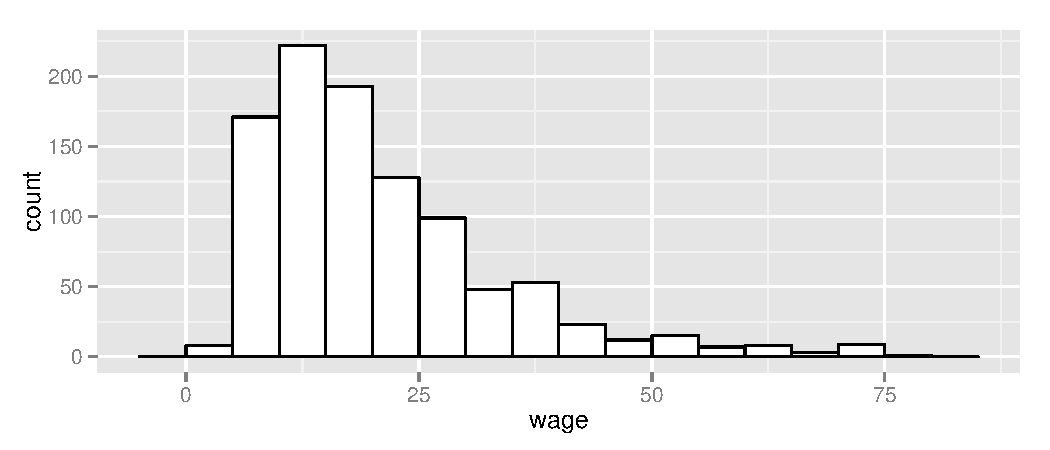
\includegraphics[width=\maxwidth]{figure/unnamed-chunk-1-1} 
\begin{kframe}\begin{alltt}
\hlkwd{library}\hlstd{(psych)}
\end{alltt}


{\ttfamily\noindent\itshape\color{messagecolor}{\#\# \\\#\# Attaching package: 'psych'\\\#\# \\\#\# The following object is masked from 'package:ggplot2':\\\#\# \\\#\#\ \ \ \  \%+\%}}\begin{alltt}
\hlkwd{describe}\hlstd{(cps4_small}\hlopt{$}\hlstd{wage)}
\end{alltt}
\begin{verbatim}
##   vars    n  mean    sd median trimmed   mad  min   max range skew
## 1    1 1000 20.62 12.83   17.3   18.67 10.27 1.97 76.39 74.42 1.58
##   kurtosis   se
## 1     2.91 0.41
\end{verbatim}
\end{kframe}
\end{knitrout}

The above plot is skewed to the right. It indicates that majority of the observations are in between the hourly wages of 5 to 40. A smaller number of observations is seen with an hourly wage above 40. The average was is 20.62 dollars per hour. The maximum earned in this sample is 76.39 dollars per hour and the lowest wage is 1.97 dollars per hour. The descriptive statistics also give median, standard deviation, range, kutosis and skewness of the wage.


\begin{knitrout}
\definecolor{shadecolor}{rgb}{0.969, 0.969, 0.969}\color{fgcolor}\begin{kframe}
\begin{alltt}
\hlcom{# Histogram of Education}
\hlkwd{library}\hlstd{(ggplot2)}
\hlkwd{ggplot}\hlstd{(cps4_small,} \hlkwd{aes}\hlstd{(}\hlkwc{x}\hlstd{=educ))} \hlopt{+} \hlkwd{geom_histogram}\hlstd{(}\hlkwc{binwidth}\hlstd{=}\hlnum{1}\hlstd{,} \hlkwc{colour}\hlstd{=}\hlstr{"black"}\hlstd{,} \hlkwc{fill}\hlstd{=}\hlstr{"white"}\hlstd{)}
\end{alltt}
\end{kframe}
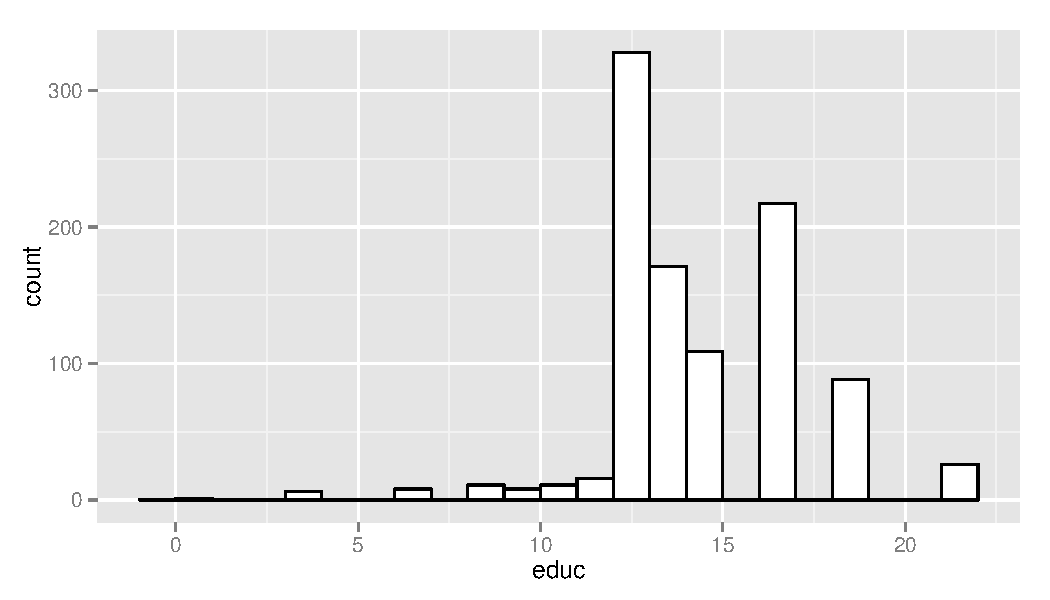
\includegraphics[width=\maxwidth]{figure/unnamed-chunk-2-1} 
\begin{kframe}\begin{alltt}
\hlkwd{library}\hlstd{(psych)}
\hlkwd{describe}\hlstd{(cps4_small}\hlopt{$}\hlstd{educ)}
\end{alltt}
\begin{verbatim}
##   vars    n mean   sd median trimmed  mad min max range  skew kurtosis
## 1    1 1000 13.8 2.71     13   13.68 1.48   0  21    21 -0.07     2.06
##     se
## 1 0.09
\end{verbatim}
\end{kframe}
\end{knitrout}

The peak at 12 years of education indicate that higher number of high school graduate. There are few observations which are less than 12 which represents high school dropout. The spike at 16 years describes the students with a four year college degree. The middle two values indicate two years of community college level degree.The rest of the histotrogram (above 16) indicate  Masters and PhD holders.The descriptive statistics also give median, standard deviation, range, kutosis and skewness of the wage.\\



(b)

\begin{knitrout}
\definecolor{shadecolor}{rgb}{0.969, 0.969, 0.969}\color{fgcolor}\begin{kframe}
\begin{alltt}
\hlstd{lm1} \hlkwb{<-} \hlkwd{lm}\hlstd{(wage}\hlopt{~}\hlstd{educ ,} \hlkwc{data}\hlstd{= cps4_small)}
\hlkwd{summary}\hlstd{(lm1)}
\end{alltt}
\begin{verbatim}
## 
## Call:
## lm(formula = wage ~ educ, data = cps4_small)
## 
## Residuals:
##     Min      1Q  Median      3Q     Max 
## -28.626  -7.816  -2.623   5.019  55.376 
## 
## Coefficients:
##             Estimate Std. Error t value Pr(>|t|)    
## (Intercept)  -6.7103     1.9142  -3.506 0.000476 ***
## educ          1.9803     0.1361  14.548  < 2e-16 ***
## ---
## Signif. codes:  0 '***' 0.001 '**' 0.01 '*' 0.05 '.' 0.1 ' ' 1
## 
## Residual standard error: 11.66 on 998 degrees of freedom
## Multiple R-squared:  0.175,	Adjusted R-squared:  0.1741 
## F-statistic: 211.7 on 1 and 998 DF,  p-value: < 2.2e-16
\end{verbatim}
\end{kframe}
\end{knitrout}

The estimated model:\\

\textbf{WAGE= -6.7103+ 1.9803EDUC}\\

The coefficient 1.9803 indicates the estimated increase in the expected hourly wage rate per year of education. The negative value of intercept represents the estimated wage rate of a worker with zero years of education. This value is meaningless as it is not possible to have a negative hourly wage rate.\\


(c)
\begin{knitrout}
\definecolor{shadecolor}{rgb}{0.969, 0.969, 0.969}\color{fgcolor}\begin{kframe}
\begin{alltt}
\hlstd{residual} \hlkwb{=} \hlkwd{resid}\hlstd{(lm1)}
\hlkwd{qplot}\hlstd{(cps4_small}\hlopt{$}\hlstd{educ, residual,} \hlkwc{xlab}\hlstd{=}\hlstr{"Education"}\hlstd{)}
\end{alltt}
\end{kframe}
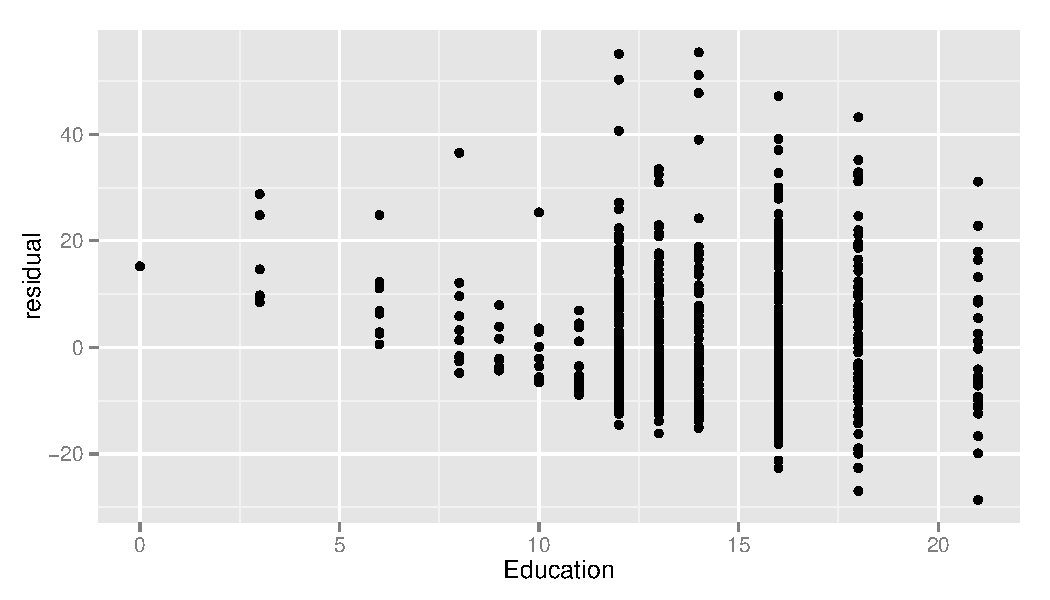
\includegraphics[width=\maxwidth]{figure/unnamed-chunk-4-1} 

\end{knitrout}

The residuals are plotted against education above. There is a pattern evident; as EDUC increases, the magnitude of the residuals also increases. It implies that the error
variance is greater for larger values of EDUC. Violation of assumption SR3 is evident here. We know that if the assumptions (SR1-SR5) hold, no particular pattern should be evident in the residuals.\\


(d)
\begin{knitrout}
\definecolor{shadecolor}{rgb}{0.969, 0.969, 0.969}\color{fgcolor}\begin{kframe}
\begin{alltt}
\hlstd{male} \hlkwb{<-} \hlstd{cps4_small[cps4_small[,} \hlstr{"female"}\hlstd{]}\hlopt{<}\hlnum{1}\hlstd{, ]}
\hlkwd{head}\hlstd{(male,}\hlkwc{n}\hlstd{=}\hlnum{3}\hlstd{)}
\end{alltt}
\begin{verbatim}
##    wage educ female midwest south west black asian
## 2 11.50   12      0       1     0    0     0     0
## 3 15.04   16      0       0     0    1     1     0
## 5 24.03   12      0       0     0    0     0     0
\end{verbatim}
\begin{alltt}
\hlstd{female} \hlkwb{<-} \hlstd{cps4_small[cps4_small[,} \hlstr{"female"}\hlstd{]}\hlopt{>}\hlnum{0}\hlstd{, ]}
\hlkwd{head}\hlstd{(female,}\hlkwc{n}\hlstd{=}\hlnum{3}\hlstd{)}
\end{alltt}
\begin{verbatim}
##     wage educ female midwest south west black asian
## 1  18.70   16      1       0     1    0     0     0
## 4  25.95   14      1       0     1    0     1     0
## 10 16.83   13      1       0     0    0     0     0
\end{verbatim}
\begin{alltt}
\hlstd{white1} \hlkwb{<-} \hlstd{cps4_small[cps4_small[,} \hlstr{"black"}\hlstd{]}\hlopt{<}\hlnum{1}\hlstd{, ]}
\hlstd{white} \hlkwb{<-} \hlstd{white1[white1[,} \hlstr{"asian"}\hlstd{]}\hlopt{<}\hlnum{1}\hlstd{, ]}
\hlkwd{head}\hlstd{(white,}\hlkwc{n}\hlstd{=}\hlnum{3}\hlstd{)}
\end{alltt}
\begin{verbatim}
##    wage educ female midwest south west black asian
## 1 18.70   16      1       0     1    0     0     0
## 2 11.50   12      0       1     0    0     0     0
## 5 24.03   12      0       0     0    0     0     0
\end{verbatim}
\begin{alltt}
\hlstd{black1} \hlkwb{<-} \hlstd{cps4_small[cps4_small[,} \hlstr{"black"}\hlstd{]}\hlopt{>}\hlnum{0}\hlstd{, ]}
\hlstd{black} \hlkwb{<-} \hlstd{black1[black1[,} \hlstr{"asian"}\hlstd{]}\hlopt{<}\hlnum{1}\hlstd{, ]}
\hlkwd{head}\hlstd{(black,}\hlkwc{n}\hlstd{=}\hlnum{3}\hlstd{)}
\end{alltt}
\begin{verbatim}
##     wage educ female midwest south west black asian
## 3  15.04   16      0       0     0    1     1     0
## 4  25.95   14      1       0     1    0     1     0
## 14 14.00   14      1       0     1    0     1     0
\end{verbatim}
\begin{alltt}
\hlstd{lm2} \hlkwb{<-} \hlkwd{lm}\hlstd{(male}\hlopt{$}\hlstd{wage}\hlopt{~} \hlstd{male}\hlopt{$}\hlstd{educ)}
\hlkwd{summary}\hlstd{(lm2)}
\end{alltt}
\begin{verbatim}
## 
## Call:
## lm(formula = male$wage ~ male$educ)
## 
## Residuals:
##     Min      1Q  Median      3Q     Max 
## -24.650  -7.558  -2.499   5.551  47.851 
## 
## Coefficients:
##             Estimate Std. Error t value Pr(>|t|)    
## (Intercept)  -3.0545     2.4935  -1.225    0.221    
## male$educ     1.8753     0.1814  10.336   <2e-16 ***
## ---
## Signif. codes:  0 '***' 0.001 '**' 0.01 '*' 0.05 '.' 0.1 ' ' 1
## 
## Residual standard error: 11.55 on 484 degrees of freedom
## Multiple R-squared:  0.1808,	Adjusted R-squared:  0.1791 
## F-statistic: 106.8 on 1 and 484 DF,  p-value: < 2.2e-16
\end{verbatim}
\begin{alltt}
\hlstd{lm3} \hlkwb{<-} \hlkwd{lm}\hlstd{(female}\hlopt{$}\hlstd{wage}\hlopt{~} \hlstd{female}\hlopt{$}\hlstd{educ)}
\hlkwd{summary}\hlstd{(lm3)}
\end{alltt}
\begin{verbatim}
## 
## Call:
## lm(formula = female$wage ~ female$educ)
## 
## Residuals:
##     Min      1Q  Median      3Q     Max 
## -29.090  -6.710  -2.918   4.132  58.008 
## 
## Coefficients:
##             Estimate Std. Error t value Pr(>|t|)    
## (Intercept) -14.1680     2.8957  -4.893 1.33e-06 ***
## female$educ   2.3575     0.2017  11.690  < 2e-16 ***
## ---
## Signif. codes:  0 '***' 0.001 '**' 0.01 '*' 0.05 '.' 0.1 ' ' 1
## 
## Residual standard error: 11.35 on 512 degrees of freedom
## Multiple R-squared:  0.2107,	Adjusted R-squared:  0.2091 
## F-statistic: 136.7 on 1 and 512 DF,  p-value: < 2.2e-16
\end{verbatim}
\begin{alltt}
\hlstd{lm4} \hlkwb{<-} \hlkwd{lm}\hlstd{(white}\hlopt{$}\hlstd{wage}\hlopt{~} \hlstd{white}\hlopt{$}\hlstd{educ)}
\hlkwd{summary}\hlstd{(lm4)}
\end{alltt}
\begin{verbatim}
## 
## Call:
## lm(formula = white$wage ~ white$educ)
## 
## Residuals:
##     Min      1Q  Median      3Q     Max 
## -27.334  -7.944  -2.353   5.147  55.054 
## 
## Coefficients:
##             Estimate Std. Error t value Pr(>|t|)    
## (Intercept)  -6.5507     2.0764  -3.155  0.00166 ** 
## white$educ    1.9919     0.1482  13.444  < 2e-16 ***
## ---
## Signif. codes:  0 '***' 0.001 '**' 0.01 '*' 0.05 '.' 0.1 ' ' 1
## 
## Residual standard error: 11.67 on 843 degrees of freedom
## Multiple R-squared:  0.1766,	Adjusted R-squared:  0.1756 
## F-statistic: 180.8 on 1 and 843 DF,  p-value: < 2.2e-16
\end{verbatim}
\begin{alltt}
\hlstd{lm5} \hlkwb{<-} \hlkwd{lm}\hlstd{(black}\hlopt{$}\hlstd{wage}\hlopt{~} \hlstd{black}\hlopt{$}\hlstd{educ)}
\hlkwd{summary}\hlstd{(lm5)}
\end{alltt}
\begin{verbatim}
## 
## Call:
## lm(formula = black$wage ~ black$educ)
## 
## Residuals:
##     Min      1Q  Median      3Q     Max 
## -16.099  -6.303  -3.557   1.760  48.031 
## 
## Coefficients:
##             Estimate Std. Error t value Pr(>|t|)    
## (Intercept) -15.0859     6.1693  -2.445   0.0161 *  
## black$educ    2.4491     0.4531   5.405  3.8e-07 ***
## ---
## Signif. codes:  0 '***' 0.001 '**' 0.01 '*' 0.05 '.' 0.1 ' ' 1
## 
## Residual standard error: 11.02 on 110 degrees of freedom
## Multiple R-squared:  0.2098,	Adjusted R-squared:  0.2027 
## F-statistic: 29.21 on 1 and 110 DF,  p-value: 3.803e-07
\end{verbatim}
\end{kframe}
\end{knitrout}

The estimated model for Male: \textbf{WAGE= -3.0545+ 1.8753EDUC}\\
The estimated model for Female: \textbf{WAGE= -14.1680+ 2.3575EDUC}\\
The estimated model for Black: \textbf{WAGE= -15.0859+ 2.4491EDUC}\\
The estimated model for White: \textbf{WAGE= -6.5507+ 1.9919EDUC}\\

In filtering white and black popular, we filtered out those who are asians. From the esimated models, it's visible that an extra year of education increases the wage rate for a black worker than for a white worker. Similar trend is visible in female workers case. Their wage rate increases with an extra year of education more than male worker.\\

(e)

\begin{knitrout}
\definecolor{shadecolor}{rgb}{0.969, 0.969, 0.969}\color{fgcolor}\begin{kframe}
\begin{alltt}
\hlstd{lmfit} \hlkwb{<-} \hlkwd{lm}\hlstd{(wage}\hlopt{~}\hlkwd{I}\hlstd{(educ} \hlopt{^}\hlnum{2}\hlstd{),} \hlkwc{data}\hlstd{= cps4_small)}
\hlkwd{summary}\hlstd{(lmfit)}
\end{alltt}
\begin{verbatim}
## 
## Call:
## lm(formula = wage ~ I(educ^2), data = cps4_small)
## 
## Residuals:
##     Min      1Q  Median      3Q     Max 
## -32.242  -7.665  -2.437   4.977  55.903 
## 
## Coefficients:
##             Estimate Std. Error t value Pr(>|t|)    
## (Intercept) 6.082831   1.023161   5.945 3.82e-09 ***
## I(educ^2)   0.073489   0.004832  15.210  < 2e-16 ***
## ---
## Signif. codes:  0 '***' 0.001 '**' 0.01 '*' 0.05 '.' 0.1 ' ' 1
## 
## Residual standard error: 11.57 on 998 degrees of freedom
## Multiple R-squared:  0.1882,	Adjusted R-squared:  0.1874 
## F-statistic: 231.3 on 1 and 998 DF,  p-value: < 2.2e-16
\end{verbatim}
\end{kframe}
\end{knitrout}

The estimated quadratic model:\\

WAGE= 6.082831+ $0.073489EDUC^2$\\

Marginal effect:\\

SLOPE= $2(0.073489)EDUC$\\

A person with 12 years of education has the estimated marginal effect of an additional
year of education on expected wage is:\\

SLOPE= 2*0.073489*12= 1.7637\\

A person with 14 years of education has the estimated marginal effect of an additional
year of education on expected wage is:\\

SLOPE= 2*0.073489*14= 2.0577\\

The linear estimated model indicated that an additional year of education is expected to increase wage by dollar 1.98 regardless of the number of years of education attained. So, the rate of change is pretty much constant. On the other hand, the quadratic model implies that the effect of an additional year of education on wage increases with the level of education.\\

(f)

\begin{knitrout}
\definecolor{shadecolor}{rgb}{0.969, 0.969, 0.969}\color{fgcolor}\begin{kframe}
\begin{alltt}
\hlstd{p} \hlkwb{<-} \hlkwd{qplot}\hlstd{(educ, wage,} \hlkwc{data} \hlstd{= cps4_small)}
\hlstd{p} \hlopt{+} \hlkwd{stat_smooth}\hlstd{(}\hlkwc{method} \hlstd{=} \hlstr{"lm"}\hlstd{,} \hlkwc{formula} \hlstd{= y} \hlopt{~} \hlstd{x,} \hlkwc{size} \hlstd{=} \hlnum{1}\hlstd{)} \hlopt{+}
\hlkwd{stat_smooth}\hlstd{(}\hlkwc{method} \hlstd{=} \hlstr{"lm"}\hlstd{,} \hlkwc{formula} \hlstd{= y} \hlopt{~} \hlkwd{I}\hlstd{(x}\hlopt{^}\hlnum{2}\hlstd{),} \hlkwc{size} \hlstd{=} \hlnum{1}\hlstd{)}
\end{alltt}
\end{kframe}
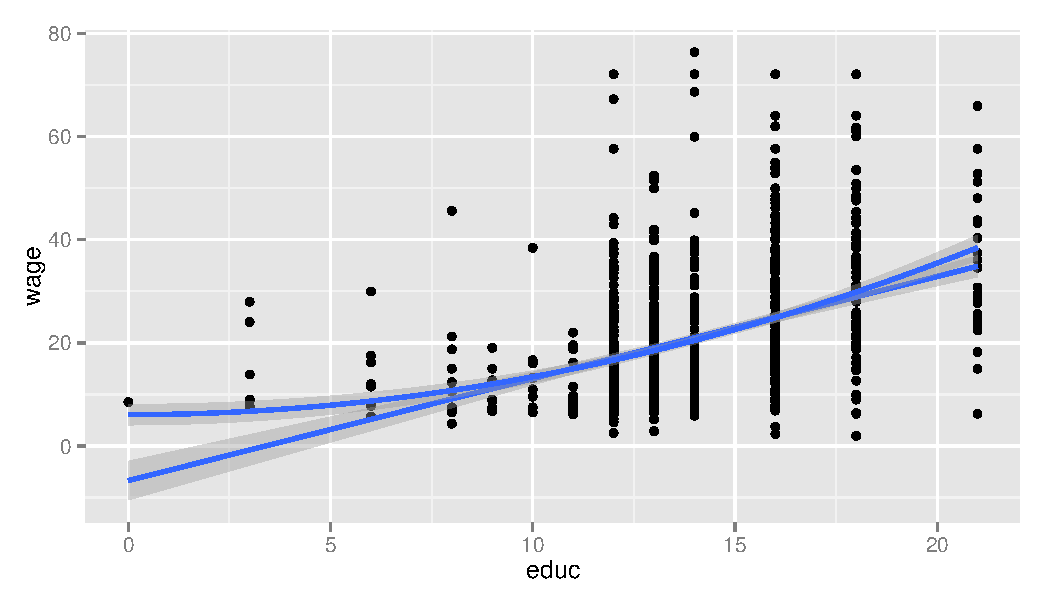
\includegraphics[width=\maxwidth]{figure/unnamed-chunk-7-1} 

\end{knitrout}

The quadratic model seems to fit the data better than the linear model equation.\\

(g)

\begin{knitrout}
\definecolor{shadecolor}{rgb}{0.969, 0.969, 0.969}\color{fgcolor}\begin{kframe}
\begin{alltt}
\hlstd{m} \hlkwb{<-} \hlkwd{log}\hlstd{(cps4_small}\hlopt{$}\hlstd{wage)}
\hlstd{cps4_small}\hlopt{$}\hlstd{logwage} \hlkwb{<-} \hlkwd{log}\hlstd{(cps4_small}\hlopt{$}\hlstd{wage)}
\hlkwd{head}\hlstd{(cps4_small)}
\end{alltt}
\begin{verbatim}
##    wage educ female midwest south west black asian  logwage
## 1 18.70   16      1       0     1    0     0     0 2.928524
## 2 11.50   12      0       1     0    0     0     0 2.442347
## 3 15.04   16      0       0     0    1     1     0 2.710713
## 4 25.95   14      1       0     1    0     1     0 3.256172
## 5 24.03   12      0       0     0    0     0     0 3.179303
## 6 20.00   12      0       0     0    0     0     0 2.995732
\end{verbatim}
\begin{alltt}
\hlkwd{ggplot}\hlstd{(cps4_small,} \hlkwd{aes}\hlstd{(}\hlkwc{x}\hlstd{=logwage))} \hlopt{+}
\hlkwd{geom_histogram}\hlstd{(}\hlkwc{binwidth}\hlstd{=}\hlnum{0.2}\hlstd{,} \hlkwc{colour}\hlstd{=}\hlstr{"black"}\hlstd{,} \hlkwc{fill}\hlstd{=}\hlstr{"white"}\hlstd{)}
\end{alltt}
\end{kframe}
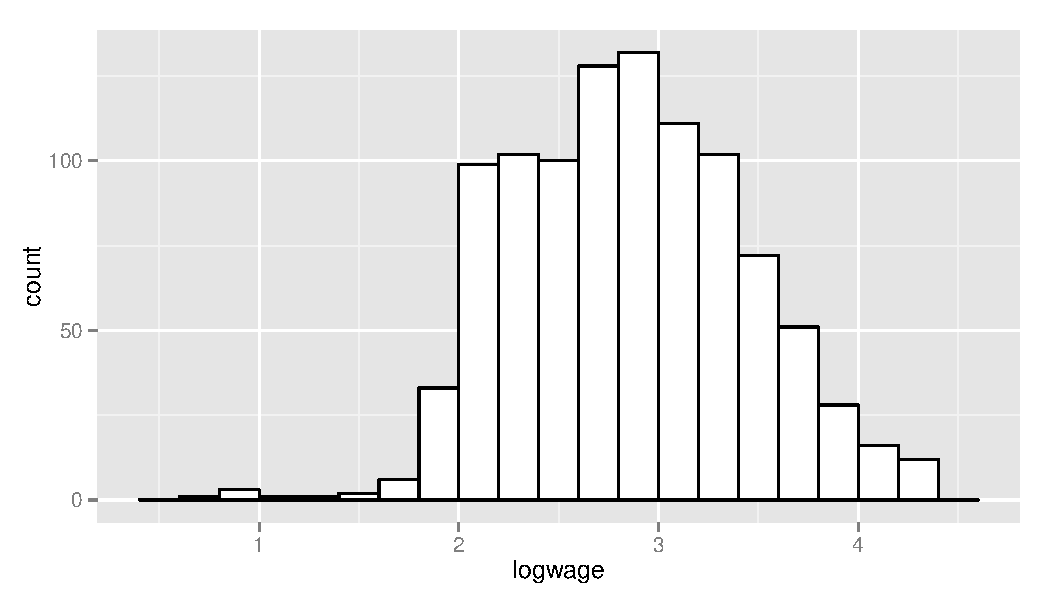
\includegraphics[width=\maxwidth]{figure/unnamed-chunk-8-1} 

\end{knitrout}

From the above plot, the histogram of log(WAGE) is more symmetrical and bell-shaped than the histogram of WAGE.\\

(h)

\begin{knitrout}
\definecolor{shadecolor}{rgb}{0.969, 0.969, 0.969}\color{fgcolor}\begin{kframe}
\begin{alltt}
\hlstd{lm6} \hlkwb{<-} \hlkwd{lm}\hlstd{(logwage}\hlopt{~}\hlstd{educ ,} \hlkwc{data}\hlstd{= cps4_small)}
\hlkwd{summary}\hlstd{(lm6)}
\end{alltt}
\begin{verbatim}
## 
## Call:
## lm(formula = logwage ~ educ, data = cps4_small)
## 
## Residuals:
##      Min       1Q   Median       3Q      Max 
## -2.55876 -0.39176  0.00699  0.36057  1.58413 
## 
## Coefficients:
##             Estimate Std. Error t value Pr(>|t|)    
## (Intercept) 1.609444   0.086423   18.62   <2e-16 ***
## educ        0.090408   0.006146   14.71   <2e-16 ***
## ---
## Signif. codes:  0 '***' 0.001 '**' 0.01 '*' 0.05 '.' 0.1 ' ' 1
## 
## Residual standard error: 0.5266 on 998 degrees of freedom
## Multiple R-squared:  0.1782,	Adjusted R-squared:  0.1774 
## F-statistic: 216.4 on 1 and 998 DF,  p-value: < 2.2e-16
\end{verbatim}
\end{kframe}
\end{knitrout}

The estimated model:\\

\textbf{log(WAGE)= 1.609444+ 0.090408EDUC}\\

Estimated marginal effect of education on WAGE is:\\

dWAGE/dEDUC=const* WAGE\\

For workers with 12  years of education the predicted wage rate:\\

$WAGE_12=exp(1.60944 + 0.090408* 12)= 14.796$\\

For workers with 14  years of education the predicted wage rate:\\

$WAGE_14=exp(1.60944 + 0.090408* 14)= 17.728$\\

The marginal effects at these values are 1.34 and 1.60 respectively.\\

\begin{knitrout}
\definecolor{shadecolor}{rgb}{0.969, 0.969, 0.969}\color{fgcolor}\begin{kframe}
\begin{alltt}
\hlstd{p} \hlkwb{<-} \hlkwd{qplot}\hlstd{(educ, wage,} \hlkwc{data} \hlstd{= cps4_small)}
\hlstd{p} \hlopt{+} \hlkwd{stat_smooth}\hlstd{(}\hlkwc{method} \hlstd{=} \hlstr{"lm"}\hlstd{,} \hlkwc{formula} \hlstd{= y} \hlopt{~} \hlstd{x,} \hlkwc{size} \hlstd{=} \hlnum{1}\hlstd{)} \hlopt{+}
\hlkwd{stat_smooth}\hlstd{(}\hlkwc{method} \hlstd{=} \hlstr{"lm"}\hlstd{,} \hlkwc{formula} \hlstd{= y} \hlopt{~} \hlkwd{exp}\hlstd{(x),} \hlkwc{size} \hlstd{=} \hlnum{1}\hlstd{)}
\end{alltt}
\end{kframe}
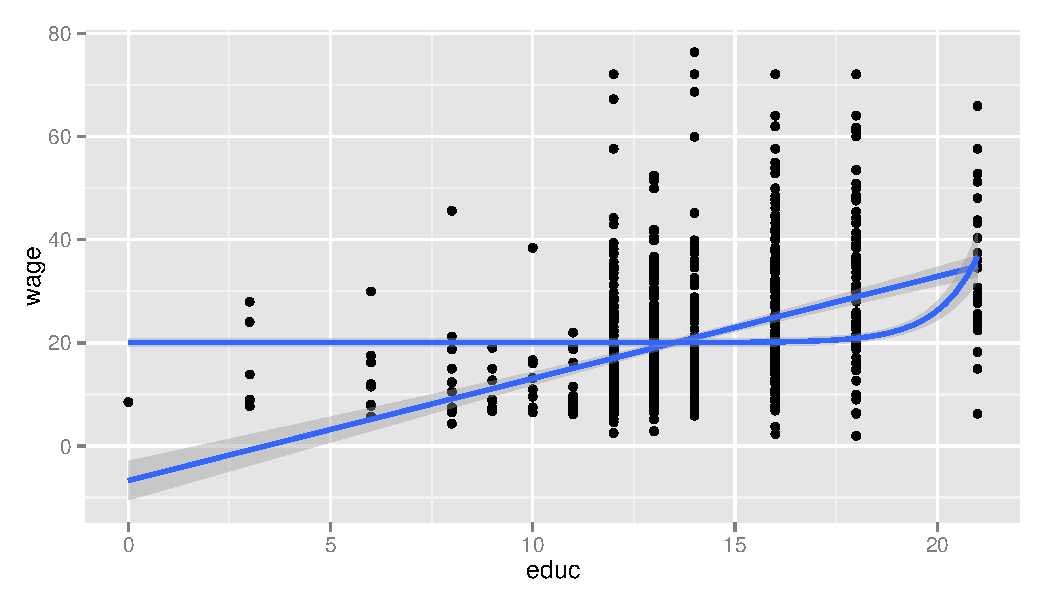
\includegraphics[width=\maxwidth]{figure/unnamed-chunk-10-1} 

\end{knitrout}

For the linear model, effect of education was estimated to be dollar 1.98. For the quadratic model, the corresponding marginal effect estimates are dollar 1.76 and dollar 2.06 respectively. The marginal effects of the log-linear model are lower.\\
\end{document}
